\section{Pegasos} \label{sec:prob3}
In this section, we use the Pegasos algorithm for soft-margin SVM binary classification of one of the 2D datasets.

\subsection{Part 1}
The Pegasos algorithm is a method to solve soft-margin SVM.
We implemented the algorithm according to the provided pseudocode, and added a bias term, $w_0$ that is incremented by $\eta_ty_i$ for misclassified sample $x_i$ each iteration.
The bias term is not penalized by the regularization.
The formulation solved by Pegasos is:
\begin{equation}\label{eq:svm_pegasos}
min_w \frac{\lambda}{2}||w||^2 + \frac{1}{N}\sum\limits_{i=1}^{N}max\{0,1-y_i(w^Tx_i)\}
\end{equation}

\subsection{Part 2}
The algorithm is applied to the same 2D dataset for several values of $\lambda$ ($\lambda = [2, 2^{-1}, 2^{-2}, 2^{-4}$), shown in~\cref{fig:3_2_lambdas}.
For large $\lambda$ (left), magnitude of $w$ is penalized heavily, so the decision boundary is not very accurate.
As $\lambda$ decreases, the regularization penalty becomes less dominant compared with accuracy, so the accuracy improves.
This intuition agrees with the objective function~\cref{eq:svm_pegasos}.

\begin{figure}
	\centering
	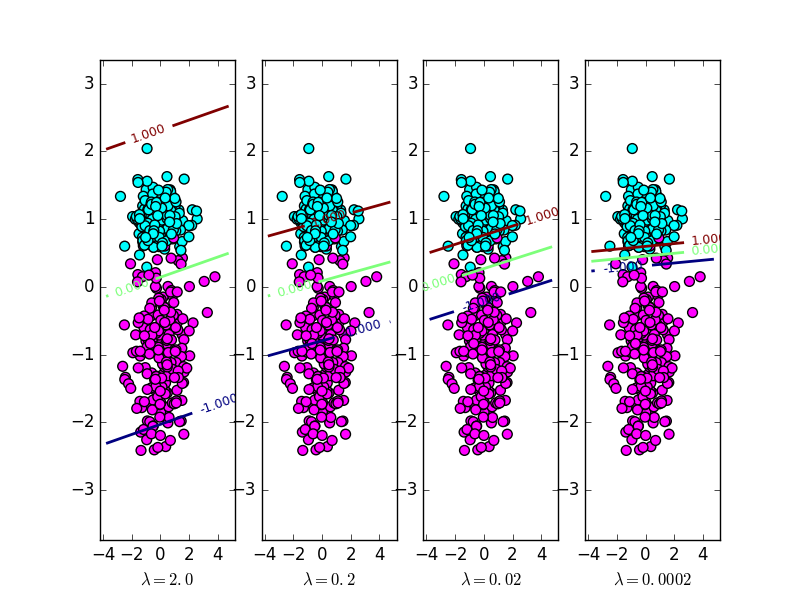
\includegraphics [trim=0 0 0 0, clip, angle=0, width=0.8\columnwidth,
	keepaspectratio]{figures/3_2_lambdas}
	\caption{The Pegasos algorithm is applied to the same dataset with four different regularization parameter values, $\lambda$. For large $\lambda$ (left), magnitude of $w$ is penalized heavily, so the decision boundary is not very accurate. As $\lambda$ decreases, the regularization penalty becomes less dominant compared with accuracy, so the accuracy improves.}
	\label{fig:3_2_lambdas} 
\end{figure}

\subsection{Part 3}
Next, we extended our implementation to handle a kernel matrix input, and tested it with a gaussian RBF kernel as in~\cref{sec:prob2}.
After learning $\alpha$, we predict the class of a new sample, $x_i$ by first calculating $c = \alpha \cdot K(X, x_i; \gamma)$, where $X$ is the entire training set and $\gamma$ is the Gaussian kernel bandwidth.
If $c > 0$, it's part of the positive class, otherwise it's the negative class.

\subsection{Part 4}
We tested our algorithm on multiple values of $\gamma$ with a fixed $\lambda=0.02$.
For large $\gamma$ (left), the kernel is very narrow, and the decision boundary overfits the data, evident in the decision boundary's jagged shape tracing around individual borderline samples.
As $\gamma$ decreases, the accuracy decreases, but the decision boundary is much less complicated.
This usually leads to better generalization to unseen data.

The number of support vectors decreases as $\gamma$ increases (192, 165, 10, 22).
This observation aligns with the decreasing complexity of the decision boundary, because each support vector affects the shape of the decision boundary.

These observations associated with increasing $\gamma$ match the trends seen in~\cref{sec:prob2} with increasing $C$.
Both implementations (Pegasos and SVM) are able to correctly classify the dataset.
Our Pegasos implementation runs much faster, making it easier to test with different parameters for increased performance.


\begin{figure}
	\centering
	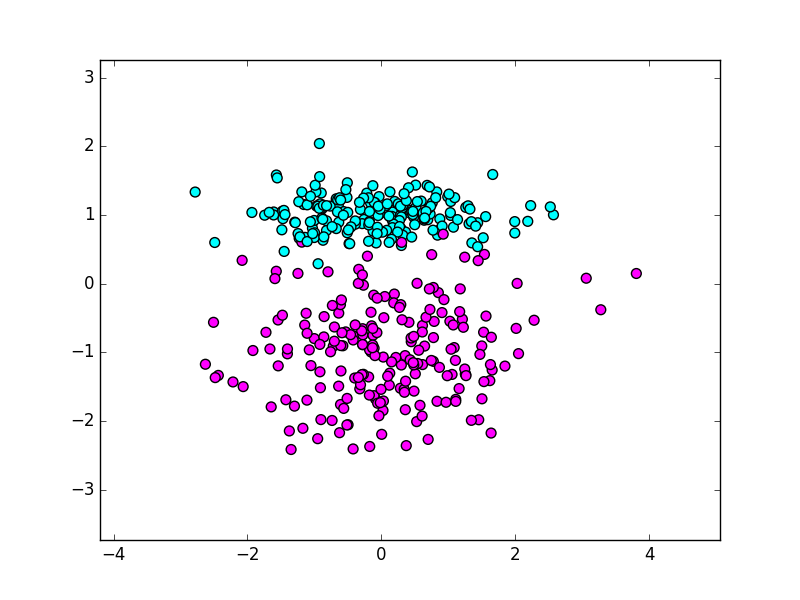
\includegraphics [trim=0 0 0 0, clip, angle=0, width=0.8\columnwidth,
	keepaspectratio]{figures/3_3_decisions}
	\caption{The Pegasos algorithm is applied to the same dataset with four different kernel bandwidth values, $\gamma = [2^2, 2^1, 2^0, 2^{-1}]$. For large $\gamma$ (left), the kernel is narrow, and the decision boundary overfits the data. As $\gamma$ decreases, the accuracy decreases, but the decision boundary is much less complicated.}
	\label{fig:3_3_decisions} 
\end{figure}